%! Author = mariuszindel
%! Date = 25.01.21

\section{Faltungscodes}


\subsection{Definition}
Zur Sicherung gegen Übertragungsfehler eingesetzt.
\begin{itemize}
    \item Leichte Implementierbarkeit der Encoder und Decoder durch Schieberegister
    \item Hohe Fehlererkennungsmächtigkeit (Bündelfehlererkennung bei zyklischen Codes)
    \item Blockbildung der zu codierenden Daten notwendig
\end{itemize}


\subsection{Encoderschaltung}
Idee: Vergangenheit berücksichtigen
\vspace{-8pt}
\begin{center}
    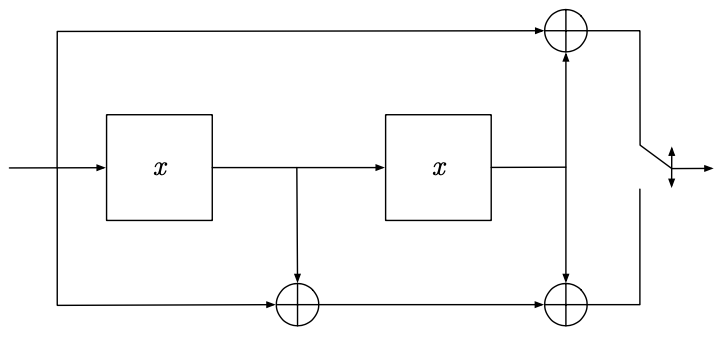
\includegraphics[scale=.33]{graphic/faltungscodes/Encoderschaltung.png}
\end{center}
\vspace{-8pt}


\subsection{Zustandsdarstellung}
\begin{center}
    \begin{tabular}{p{0.7cm} | p{0.7cm}  p{.7cm} p{.4cm} | p{.3cm} p{.1cm} | p{1cm}}
        \hline
        Eingang & Zustand & \multicolumn{2}{p{.1cm}|}{Schieberegister} & \multicolumn{2}{p{.1cm}|}{Ausgang} & Nächster Zustand \\
        \hline
        \hline
        0   &   $S_0$   &   0   &   0   &   0   &   0   &   $S_0$\\
        1   &   $S_0$   &   0   &   0   &   1   &   1   &   $S_1$\\ \hline
        0   &   $S_1$   &   1   &   0   &   0   &   1   &   $S_2$\\
        1   &   $S_1$   &   1   &   0   &   1   &   0   &   $S_3$\\ \hline
        0   &   $S_2$   &   0   &   1   &   1   &   1   &   $S_0$\\
        1   &   $S_2$   &   0   &   1   &   0   &   0   &   $S_1$\\ \hline
        0   &   $S_3$   &   1   &   1   &   1   &   0   &   $S_3$\\
        1   &   $S_3$   &   1   &   1   &   0   &   1   &   $S_3$\\
    \end{tabular}
\end{center}
\begin{enumerate}
    \item Tabelle mit Eingangsbits und Zuständen erstellen
    \item Ausgänge aufschreiben:
    \begin{itemize}
        \item 1. Ausgangsbit (g1) addieren Eingangsbit $+$ zweite Schieberegisterbit (mod 2)
        \item 2. Ausgangsbit (g2) addieren Eingangsbit $+$ beide Schieberegisterbit (mod 2)
    \end{itemize}
    \item Nächsten Zustand bestimmen
    \begin{itemize}
        \item Schieben der Schieberegister: Eingangsbit und erste Schieberegisterbit übernommen.
    \end{itemize}
    \item Zustandsdiagramm Zeichnen:
\end{enumerate}
\vspace{-8pt}
\begin{center}
    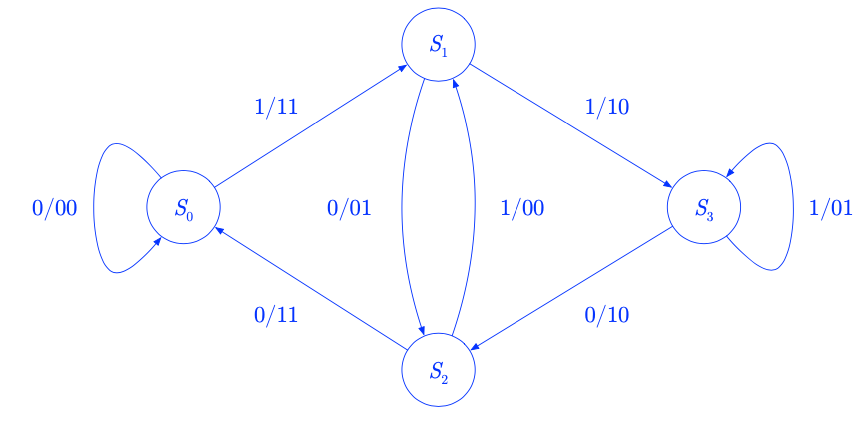
\includegraphics[width=\linewidth]{graphic/faltungscodes/Zustandsdiagramm.png}
\end{center}
\vspace{-8pt}



\subsection{Diverse Berechnungen}

\subsubsection{Generatorpolynome}
Hier genau zwei Polynome, da im Faltungscoder genau zwei ''Ausgänge''.\\
$g_1(x) = 1 + x^2$ (weil hinter 2. Speicher)\\
$g_2(x) = 1 + x + x^2$ (weil hinter 1. und 2. Speicher)

\subsubsection{Tailbits}
anz. Tailbits = anz. Speicherplätze

\subsubsection{Codergedächnis}

\subsubsection{Impulsantwort der Decoderschaltung}
\begin{enumerate}
    \item Beispielnachricht (${u[n]}$) einfügen (länge = anz. Speicher + 1)
    \item Durchspielen
\end{enumerate}

\subsubsection{Anzahl Zustände}
$2^n$, n=Speicherplätze

\subsubsection{Anzahl Bits für Berechnung}
Anz. = anz. Speicherplätze + aktuelle Bit

\subsubsection{Coderate bestimmen}
Anz. Ausgangsbits / Anz. Eingangsbits

\subsubsection{Block- Coderate}
% TODO
$R=\frac{Eingabebits}{Anz. Ausgänge \cdot(Eingabebits + Speicherblöcke)}$





\subsection{Übertragunsfunktion}
\subsection{Trellisdiagramm}
